%---------------------------------------------------------------------------------------------------
% Hauptteil
%---------------------------------------------------------------------------------------------------
%\newpage
%%\part{Hauptteil}

% Kapitel 1: Von der Integration zur Inklusion - eine Begriffserkl�rung 
\chapter{Sozial-emotionale Kompetenzen: Begriffserkl\"arung}
  \section{Emotionale Kompetenz}
    \begin{flushleft}
      �berfordert
    \end{flushleft}

  \section{Soziale Kompetenz}
    \begin{flushleft}
    \end{flushleft}

  \section{Emotionale Kompetenz}
    \begin{flushleft}
    \end{flushleft}
      \subsection{Konflikte}
        \begin{flushleft}
        \end{flushleft}

  \section{Sozial-emotionale Kompetenzen ein lebenslanger Prozess}
    \begin{flushleft}
    \end{flushleft}

     
  %   \begin{flushleft}
  %     Der noch relative neue Begriff Inklusion, ist derzeit Bestandteil \gls{Bewegungsangbote} heftiger Debatten in der Fach�ffentlichkeit - es zieht so wohl Bef�rworter als auch Gegner nach sich. Mitverantwortlich f�r diese Unstimmigkeiten sind sowohl die unterschiedlichen �bersetzungen und Ableitungen dieses Begriffes, als auch die konzeptionelle Unterscheidung zum Begriff Integration. Doch um Inklusion und ihre Verbindung zur Integration zu verstehen, ist f�rderlich wenn wir historisch einige Schritte zur�ck gehen.\citep[vgl.][S.~18f]{EmotionaleK2008}
  %   \end{flushleft}
  %   
  %   \begin{flushleft}
  %     \enquote{\textit{Mit dem Begriff der Inklusion verbindet sich in der Fr�hp�dagogik der Gedanke, allen Kindern das Aufwachsen in einer Kindertageseinrichtung zu erm�glichen.} (Zitat: \citep[vgl.][S.~9]{Mittendrin2011}}
  %   \end{flushleft}
  % 
  %   \begin{flushleft}
  %     Inklusion ist aus p�dagogischer Sicht keine Erfindung des 21 Jahrhunderts, den Weg f�r Inklusion bzw. Inklusionsp�dagogik ebneten die Integrationsbestrebungen der 1970er Jahre des letzten Jahrhunderts. Hier war das Bestreben, die gemeinsame Erziehung und Bildung von Kindern mit und ohne besonderen F�rderbedarf in Kindertagesst�tten und Schulen. Diesen Fortschritt verdanken wir Eltern, die f�r ihre Kinder das Recht erstritten Regelkindertageseinrichtungen besuchen zu d�rfen und nicht wie es �blich war, Kinder mit Behinderungen in Sondereinrichtungen unterzubringen.\citep[vgl.][S.~9]{Mittendrin2011}
  %   \end{flushleft}
  %   \newpage
  %   \begin{flushleft}
  %     Das Bestreben alle Kinder gemeinsam zu erziehen und zu bilden ist bis heute nicht voll und ganz umgesetzt worden. Zwar ist der Inklusionsanteil in Kindertageseinrichtung mit 61,5\% im Vergleich zu nur 18,4\% in der Schule\footnote{2 Grundschulen : 33,6\%, weiterf�hrende Schulen 14,9\% Inklusionsanteil= Anteil der Kinder mit sonderp�dagogischen F�rderbedarf, die mit Kindern ohne F�rderbedarf zusammen in den Bildungseinrichtungen sind} recht hoch, doch es sollte nicht aus den Augen verloren werden, dass der Exklusionsanteil in Kindertageseinrichtungen immer noch 38,5\% betr�gt\citep[vgl.][S.~16]{InkiKte2011}. Im Gro�en und Ganzen kann man sagen, dass der Elementarbereich, der Bereich des deutschen Bildungssystems ist, in dem Inklusion am weitesten fortgeschritten ist, wohingegen sie dann in den folgenden Stufen immer mehr abnimmt. Gr�nde liegen unter anderem darin, dass in der Primarstufe teilweise noch Schuleingangsuntersuchungen existieren, die wiedergeben, ob ein Kind schulf�hig ist und wenn dies nicht der Fall ist, wird dieses Kind entweder zur�ckgestellt oder in eine Sonderschule �berwiesen.\citep[vgl.][S.~15]{InkidFr2010}
  %   \end{flushleft}
  % 
  % \section{Abgrenzung zur Integrationsp�dagogik}
  %   \begin{flushleft}
  %     Betrachtet man Inklusion bzw. inklusive P�dagogik unabh�ngig von den Debatten, so kann sie als Notwendigkeit f�r eine Neubetrachtung, Weiterf�hrung und Modifizierung von Integration gesehen werden.\citep[vgl.][S.~19]{Gemeinsam2012} Das Ziel von Integration ist es Kinder in das System zu holen, da davon einer Zwei-Gruppen-Klassifizierung ausgegangen wird. Au�erdem stellt die Integrationsp�dagogik das Kind mit besonderen Bed�rfnissen isoliert in den Mittelpunkt. Wohingegen Inklusionsp�dagogik von einer heterogenen (vgl. Abschnitt \ref{sec:2_2}) Lerngruppe ausgeht, die gemeinsame Interaktion ist hier das Ziel. Somit l�sst Inklusion es gar nicht so weit kommen, dass Menschen aus dem System ausgeschlossen werden.\citep[vgl.][]{DownSyndrom2012} Damit verk�rpert Inklusion genau das Gegenteil von Exklusion (Ausgeschlossensein). Eine weitere Form ist die Separation, ihr Ziel ist die h�chst m�gliche Homogenit�t von Gruppen. Ein Produkt der Separation ist die Sonderp�dagogik. Diese stellt sich in folgender Abbildung dar:\citep[vgl.][S.~18]{Gemeinsam2012}
  %   \end{flushleft}
  %   
  %   \begin{center}
  %     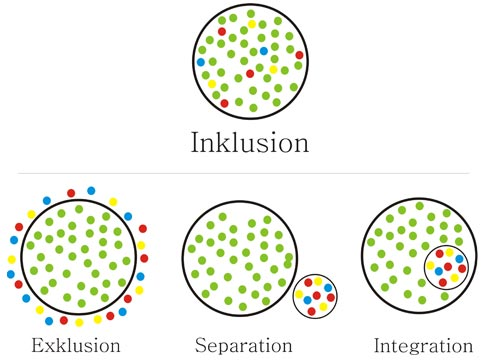
\includegraphics[width=.60\textwidth]{grafik/inklusion.jpg}
  %     \captionof{figure}[Die Abbildung stellt die verschiedenen Formen die Gesellschaft annehmen kann dar]{Die Abbildung stellt die verschiedenen Formen die Gesellschaft annehmen kann dar \citep[vgl.][]{Inkolpe2012}}
  %     \label{fig:inklusion}
  %   \end{center}
  %   
  %   \begin{flushleft}
  %     Des Weiteren geht Inklusion davon aus, dass alle Menschen ein Recht auf gemeinsame Erziehung und Bildung haben. Der Anspruch besteht darin Schulen und Kindertagesst�tten so zu gestalten und auszustatten, dass kein Kind bzw. Mensch (dies gilt auch f�r Mitarbeiter und Eltern) ausgeschlossen wird. Hierf�r ben�tigt es ein Zusammenspiel von vielen Parteien, denn jeder --- Kinder, P�dagogen, Eltern, Verwaltung und Politik tr�gt dazu bei, dass Inklusion  gelebt werden kann \citep[vgl.][S.~5]{IndexInk2007}. Obendrein verlangt Inklusion Ausgrenzung zu  vermeiden und Barrieren f�r Spiel, Lernen und Partizipation zu reduzieren. Bei der Vermeidung von Ausgrenzungen ist es wichtig niemanden in eine \enquote{Schublade zu stecken}, denn jedes Kind ist anderes und hat seine eigene Pers�nlichkeit und Begabungen. Jedes Kind bringt Erfahrungen und Eigenschaften mit, die es pr�gen und gepr�gt haben das macht jedes Kind einzigartigen. Doch die Einzigartigkeit kann sich nur in einer wertsch�tzenden Gemeinschaft bzw. Gesellschaft optimal entwickeln und entfalten. So ist das Ziel von inklusiver P�dagogik eine Gemeinschaft zu werden in der Heterogenit�t (vgl. Abschnitt \ref{sec:2_2}) als die Norm gesehen wird. Teilhabe und Chancengleichheit sind hier Schl�sselw�rter.\citep[vgl.][S.~9f]{Vielfalt2012}
  %     \newline
  %     Inklusion zu 100\% durchzusetzen und umzusetzen ist ein Ideal was nat�rlich erstrebenswert ist, aber bei l�ngerer Betrachtung nicht umsetzbar ist. Denn f�r eine v�llige Inklusion m�ssten alle Ausgrenzungsmechanismen und -prozesse verband werden. Dies scheint undenkbar, denn sowie auch inklusiven P�dagogik im st�ndigen Wandel ist, so sind auch Ausgrenzungsprozesse im st�ndigen Wandel und schwer zu �berwinden. Trotz allem sollte es aber nicht zur Resignation f�hren, sondern anspornen Inklusion zu leben.\citep[vgl.][S.~15]{IndexInk2007}
  %   \end{flushleft}


\newpage

% Kapitel 2: Fehldeutungen und Chancen von Inklusion				
\chapter{Erwerb und F�rderung von sozial-emotionalen Kompetenzen durch Spiel und Bewegung}
  \section{Was wird unter Spiel verstanden}
    \begin{flushleft}
    \end{flushleft}

  \section{Bewegung - Bet�tigungs- und Ausdrucksform von Kindern}
    \begin{flushleft}
    \end{flushleft}

  \section{Durch Spiel und Bewegung sozial-emotionale Kompetenzen erwerben}
    \begin{flushleft}
    \end{flushleft}
    \subsection{Die Bedeutung vom Spiel mit Gleichaltrigen f�r die sozial-emotionale Entwicklung bei Kindern}
      \begin{flushleft}
      \end{flushleft}

  \section{Durch Spiel und Bewegung sozial-emotionale Entwicklung f�rdern}
    \begin{flushleft}
    \end{flushleft}
    \subsection{Projekt: F�rderung sozial-emotionaler Kompetenzen in Bewegung}
      \begin{flushleft}
      \end{flushleft}


% \chapter{Fehldeutungen und Chancen von Inklusion}
%   \section{Rechtliche Grundlage}
%     \begin{flushleft}
%       Erste Schritte und Rahmenbedingungen f�r Inklusion zu schaffen und diese auch auf gesellschaftlicher Ebene zu erreichen, gelang im Verlauf der 2006 stattfindenden UNESCO- Weltmeisterkonferenz. Dies wurde als Auftrag an alle Mitgliedstaaten formuliert. In Deutschland wurden 2009 die Leitlinien f�r inklusive Bildung ver�ffentlicht.\citep[vgl.][S.~11]{Vielfalt2012} Die Umsetzung von inklusiver Fr�hp�dagogik verlangt mehr als nur eine rechtliche Entscheidung, sowohl auf nationaler, wie auch auf internationaler Ebene. Es wird vielmehr ein weites Spektrum an rechtlichen Dokumenten ben�tigt um diesem facettenreichen und komplexen Thema gerecht zu werden. Wichtig f�r Inklusive P�dagogik in Deutschland wie auch international sind die UN-Menschenrechtskonvention, die den Grundstein f�r Inklusion und inklusives Denken bildet. Des Weiteren spielen noch die UN-Kinderrechtkonvention, die UN-Behindertenkonvention, die UNESCO-Weltmeisterkonferenz und speziell f�r Deutschland das Kinder - und Jugendhilfegesetz eine wichtige Rolle.\citep[vgl.][S.~16]{InkidFr2010} Im weiteren Verlauf werde ich auf einige Punkte weiter eingehen und sie erkl�ren.
%     \end{flushleft}
%     \subsection{UN-Menschenrechtskonvention}
%       \begin{flushleft}
%         Die UN - Menschenrechtskonvention vom 10.Dezember 1948 ist das Fundament der inklusiven Bildung und Erziehung und wurde in weiteren Konventionen konkretisiert. Schon in der vom 10.Dezember 1948 verabschiedeten Resolultion 217 A (III) der Generalversammlung, ist Bildung ein Menschenrecht.\citep[vgl.][]{unmenschen2012}
%       \end{flushleft}
% 
%     \subsection{UN-Kinderrechtskonvention}
%       \begin{flushleft}
%         Im Rahmen der UN-Kinderrechtskonvention, die am  20. November.1989 stattfand, wurde das �bereinkommen �ber die Rechte der Kinder verabschiedet.
%         Die �bereinstimmung der Kinderrechtskonvention wurde von Deutschland 1990 unterzeichnet und trat dann im Jahre 1992 in Kraft.\citep[vgl.][S.~25]{Mittendrin2011}
%         Doch die Fragen sind- Was besagt die Konvention und wie genau sehen die Rechte der Kinder aus? Verbot von Diskriminierung auf Grund von Behinderung von Kindern oder deren Eltern, Chancengleichheit unabh�ngig von Herkunft und sozialen Status. Au�erdem wird allen Kindern (Kinder mit Behinderungen sind damit ebenfalls gemeint) das Recht auf Bildung zugesprochen\citep[vgl.][]{unkinder1992}.
%       \end{flushleft}
%       \begin{flushleft}
%         Bis zum Jahre 2010 behielt sich Deutschland vor Unterschiede bei der Umsetzung der Rechte inl�ndischer und ausl�ndischer Kindern zu machen. Hierbei f�hrte es zu einer starken Benachteiligung von Fl�chtlingskindern in vielerlei Hinsicht. Vor allem aber in den Bereichen Bildung, Kinder- und Jugendhilfe und medizinischer Versorgung. Von Chancenungleichheiten in den Bereichen Bildung und Ausbildung sind im gro�en Ma�e Kinder die von Armut betroffen sind, Kinder die von Behinderung betroffen sind und Kinder mit einem Migrationshintergrund betroffen. Hierf�r sprechen auch die Zahlen das nur 84\% von Kindern mit Migrationshintergrund eine fr�hp�dagogische Einrichtung besuchen.\citep[vgl.][S.~26]{Mittendrin2011}
%       \end{flushleft}
%       \begin{flushleft}
%         Deutschland konnte trotz des Aktionsplans die Einhaltung und vollst�ndige Umsetzung der Kinderrechte nicht voll und ganz gew�hrleisten. Mit Schuld an der Misere ist die Nicht-Verankerung der Kinderrechte in der deutschen Verfassung, denn es verliert dadurch an Aufmerksamkeit des Staates und der Gesellschaft.\citep[vgl.][S.~26]{Mittendrin2011}
%         \newline
%         Am 1.August 2012 wurde ein Zusatzprotokoll erstellt, welches die Rechte der Kinder verbessern soll. Kinder und Jugendliche k�nnen auf internationaler Eben gegen den Staat bei Widrigkeiten gegen das Kinderrecht Beschwerde einlegen. Doch daf�r m�ssen mindestens 10 Staaten das Protokoll unterschreiben, damit es �berhaupt in Kraft tritt.
%       \end{flushleft}
%     \subsection{UN-Behindertenrechtskonvention}
%       \begin{flushleft}
%         In Deutschland wurde inklusive P�dagogik stark von den �bereinkommen der UN-Behindertenrechtkonvention beeinflusst \citep[vgl.][S.~9]{InkiKte2011}. Hier haben sich 2006 die Vereinten Nationen auf ein Abkommen geeinigt. Seit 2010 ist es auch auf Bundeseben rechtskr�ftig. Im Mittelpunkt der Behindertenrechtskonvention stehen die Chancengleichheit und die Diskriminierung von Menschen mit Behinderung. Sie lehnt damit an die Kinderrechtskonvention an bzw. f�hrt einige Punkte weiter aus.\citep[vgl.][S.~26]{Mittendrin2011}
%         \newline
%         Im Artikel 24 erkennen die Vereinten Nationen an, das Menschen mit Behinderungen ein Recht auf Bildung haben. Damit ein lebenslanges Lernen auch gew�hrleistet werden kann, versichern die Vereinten Nationen ein integratives  (im Englischen inclusive) Bildungssystem. Es geht bei der Konvention nicht darum Menschen mit Behinderungen einen Platz in der Gesellschaft und ihren Institutionen zu schaffen, es geht viel mehr darum die Gesellschaft und ihre verschiedenen Institutionen so zu gestalten, dass sie auf die Bed�rfnisse der menschlichen Vielfalt reagieren, agieren und diese anerkennen.\citep[vgl.][S.~27]{Mittendrin2011}
%       \end{flushleft}
%       \begin{flushleft}
%         Erw�hnt werden muss, dass alle Vertragsstaaten zwar die Verpflichtung haben die Rechte in einem gewissen Rahmen umzusetzen, es aber nicht die M�glichkeit besteht diese einzuklagen solange es nicht auf Bundesebene umgesetzt wurde. Doch haben auch hier die Bundesl�nder wiederum verschiedene Vorgehensweisen bzw. Gesetzes�nderungen und somit sieht auch die Umsetzung unterschiedlich aus.\citep[vgl.][S.~16]{InkidFr2010}
% 
%         In Deutschland gehen rund die H�lfte der Kinder �ber drei Jahren mit besonderen F�rderbedarf in einen Regelkindergarten bzw. besuchen eine integrative Kindertageseinrichtung. Doch sieht man genauer hin, kann man gro�e Unterschiede in den einzelnen Bundesl�ndern erkennen\ref{fig:verteilung}. So besuchen in Th�ringen alle Kinder �ber drei Jahre mit besonderen F�rderbedarf, die eine Institution besuchen, eine integrative Kindertageseinrichtung bzw. einen Regelkindergarten wobei in Niedersachsen nur 42,1\% eine integrative Ma�nahme besuchen. Obwohl dies in Deutschland gesetzliche geregelt ist.\citep[vgl.][]{13kuj2009}
%         \newline
%         \enquote{\textit{F�r Kindertagesst�tten besteht �ber den Grundsatz der uneingeschr�nkten Teilhabe (� 4 Absatz 3, � 19 Absatz 3 SGB IX) hinaus ein integrativer F�rderauftrag (� 22a Absatz 4 Sozialgesetzbuch VIII). Demnach sollen Kinder mit und ohne Behinderung grunds�tzlich in Gruppen gemeinsam gef�rdert werden.}}(Zitat: \citep[][]{Unesco2012})
% 
%       \end{flushleft}
%       \begin{center}
%         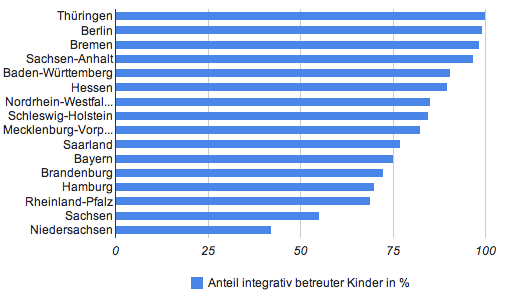
\includegraphics[width=.75\textwidth]{grafik/verteilung.png}
%         \captionof{figure}[Verteilung integrativ betreuter Kinder �ber die deutschen Bundesl�nder]{Verteilung integrativ betreuter Kinder �ber die deutschen Bundesl�nder \citep[vgl.][]{13kuj2009}}
%         \label{fig:verteilung}
%       \end{center}
%     \subsection{UNESCO Weltministerkonferenz}
%       \begin{flushleft}
%         Mit Teilnehmern aus mehr als 150 L�ndern fand 2008 die Abschlusssitzung der UNESCO Weltministerkonferenz zum Thema Bildung f�r alle in Genf statt. Es ist das gr��te und wichtigste Programm zum Thema Bildung. Das Ziel ist, dass alle Menschen zu einer qualitativ hochwertigen Bildung kommen, unabh�ngig  von Geschlecht, Hautfarbe, Religion, ihres sozio�konomischen Status\footnote{Der sozio�konomische Status bezeichnet Merkmalen menschlicher Lebensumst�nde. Dazu geh�ren beispielsweise: Bildung, Beruf, Besitz (auch kultureller Besitz) und Einkommen., url: \url{http://de.wikipedia.org/wiki/Sozio�konomischer_Status}} oder ihres besonderen F�rderbedarfs. Der Begriff Inklusion beschreibt und verk�rpert diesen Wunsch bzw. dieses Vorhaben am besten. Des Weiteren wird in der Abschlusserkl�rung der UNESCO Weltministerkonferenz, gefordert dass Bildungssysteme inklusiv sein sollen und das Bildungssysteme Vielfalt als Ressource sehen sollen.
%         \newline 
%          Die Leitlinien von dem Programm Bildung f�r alle unterst�tzen Staaten, Inklusion in ihrer Bildungspolitik und in ihren Bildungssystemen aufzunehmen . Die deutsche Fassung  \enquote{Inklusion: Leitlinien f�r die Bildungspolitik} macht die Erkenntnisse der internationalen Beratungen �ber inklusive Bildung in Deutschland zug�nglich. Obendrein bietet es einen �berblick �ber das Konzept der Inklusion sowie die rechtlichen Instrumente. Den Staaten werden  konkrete Leitfragen an die Hand gegeben. Diese geben Hilfestellung bei der Analyse des Bildungssystems. So kann z.B. Deutschland schauen wo es im Bildungssystem noch Verbesserungspotential gibt und wie der Wandel zur Inklusion vorrangetrieben werden kann. Des Weiteren wird aufgezeigt wie wichtig es ist, den Inklusionsgedanken in Deutschland zu st�rken.
%          \newline
%         Au�erdem besuchen ausnahmslos viele Kinder mit Migrationshintergrund F�rderschulen, die meist ohne ad�quaten Abschluss von der Schule abgehen. Folglich bleibt ihnen die Teilhabe und Chancengleichheit verweigert. Deutschland muss noch einiges Leisten um von einer Bildungsgerechigkeit in diesem Land sprechen zu k�nnen. Die UNESCO Leitlinien zeigen jedoch auf wie Deutschland dem Ziel von einer Inklusivenbildung n�her kommt.\citep[vgl.][]{UNESCO2010}
%       \end{flushleft}
%     \subsection{Gesetzliche Grundlagen in Deutschland}
%       \begin{flushleft}
%         In Deutschland bildet das am 1 Januar 1990 in Kraft getretene Kinder- und Jugendhilfegesetz (Achte Buch Sozialgesetzbuch (SGB VIII)) die Grundlage f�r einen deutschlandweiten gesetzlichen Rahmen der Kinderbetreuung. Das Kinder- und Jugendhilfegesetz regelt unter anderem die Bildung, Betreuung und Erziehung von Kindern in Kindertagesst�tten. Doch auch hier gibt es unterschiedliche Auslegungen in den sechzehn Bundesl�ndern. Zur Weiterentwicklung der Kinder und Jugendhilfe und zum Ausbau der Tagesbetreuung wurde das Tagesbetreuungsgesetz entwickelt.\citep[vgl.][]{Mittendrin2011} Das am 1.1.2005 in Kraft getretene Gesetz, dient unter anderem dem Ausbau der Betreuung von Kindern unter drei Jahren, h�heren Qualifikationsanforderungen und Qualit�tsentwicklung in der fr�hkindlichen Bildung.\citep[vgl.][]{TAG2004} Hervorgehoben werden die Verbesserungen und Bedeutung von Bildung, Erziehung und Entwicklung in der Fr�hp�dagogik. Dies soll Kindern gleichere Startbedingungen erm�glichen. Die Betreuungsquote der Kinder im Alter von unter drei Jahren ohne Migrationshintergrund liegt bei 30 Prozent. Bei Kindern mit Migrationshintergrund ist die Betreuungsquote mit 14 Prozent nicht einmal halb so hoch.\citep[vgl.][]{Dritter2012}
%       \end{flushleft}
%       \begin{flushleft}
%         Eine weitere Gesetzs�nderung bildet in der Bundesrepublik einen zentralen Baustein beim Ausbau der Kindertagesbetreuung. Das am 16. Dezember 2008 in Kraft getretene Kinderf�rderungsgesetz (Kif�G) soll den Ausbau eines qualitativ hochwertigen Betreuungsangebotes beschleunigen, sowie ein bedarfsgerechtes und qualitativ hochwertiges Angebot f�r Kinder unter drei Jahren gew�hren.\citep[vgl.][]{BMFSFJ2010}
%         Das Ziel ist es unter anderem, dass nach Abschluss der Ausbauphase (13. Juli 2013 ) ALLE Kinder unter drei einen Rechtsanspruch auf einen Betreuungsplatz haben. Von der Gesetzes�nderung sollen vor allem Kinder mit Entwicklungsgef�hrdung profitieren. Des Weiteren wird die Wichtigkeit der fr�hkindlichen Betreuung untermauert, sie verliert somit immer mehr ihren Stempel \enquote{nur eine Betreuungsst�tte} und erlangt den Status ein pr�ventive Funktion zu haben und als erste Bildungsst�tte. Kinder unter drei Jahren mit besonderen F�rderbedarf werden von dem Recht eine Regelkindertagesbetreuung besuchen zu d�rfen nicht ausgeschlossen.\citep[vgl.][S.~30f]{Mittendrin2011} Doch da stellt sich die Frage wie der Behinderungsbegriff in Deutschland definiert wird --- das Sozialgesetzbuch IX besagt: \enquote{Menschen sind behindert, wenn ihre k�rperliche Funktion, geistige F�higkeit oder seelische Gesundheit mit hoher Wahrscheinlichkeit l�nger als sechs Monate von dem f�r das Lebensalter typischen Zustand abweichen und daher ihre Teilhabe am Leben in der Gesellschaft beeintr�chtigt ist. Sie sind von Behinderung bedroht, wenn die Beeintr�chtigung zu erwarten ist.}( �2 Absatz 1 SGB IX,)\citep[vgl.][]{Beh2012}
%       \end{flushleft}
% 
%       \begin{flushleft}
%         Eine Behinderung wird bei Kindern unter drei eher selten diagnostiziert. Doch auch Kinder bei denen keine eindeutige Diagnose einer Behinderung vorliegt bzw. der Verdacht besteht von Behinderung bedroht zu sein, bekommen die gleichen Rechte wie Kinder die behindert sind.\citep[vgl.][S.~31]{Mittendrin2011} Hier wirkt der sonderp�dagogischer F�rderbedarf. F�r seine Feststellung muss ein Gutachten erstellt werden. Unter anderem wird festgelegt, ob und welche Ma�nahmen das Kind f�r eine uneingeschr�nkte Teilhabe in einer Kindertagesst�tte und f�r das sp�tere Leben ben�tigt.\citep[vgl.][]{Schul2012} In vielen Einrichtungen bietet der sonderp�dagogische F�rderbedarf ebenfalls kulturelle und politische Rahmenbedingungen und beeinflusst deren Handhabe. Auf diese Weise werden Gutachten �ber sonderp�dagogischen F�rderbedarf genutzt um individuelle F�rderpl�ne zu erstellen. Im Weiteren werden die Gutachten f�r Rechenschaftsberichte der Einrichtung �ber ihre Ausgaben f�r besonderen F�rderbedarf genutzt.\citep[vgl.][S.~17]{IndexInk2007}
%       \end{flushleft}
% 
%   \section{Dimensionen -- ein Diskurs der P�dagogik der fr�hen Kindheit}\label{sec:2_2}
%     \begin{flushleft}
%       In Kindertagesst�tten ist eine Vielfalt an Pers�nlichkeiten vertreten, die alle zu ihrem Recht kommen wollen. Hierzu geh�ren nicht nur die Kinder die eine Einrichtung besuchen, sondern auch ihre Familien spielen eine zentrale Rolle im Heterogenit�tsverst�ndnis. Denn jede Familie bringt unterschiedliche Erwartungen, W�nsche, Vorstellungen und Erfahrungen und Lebensweisen mit, die sie von anderen unterscheidet und die sie gepr�gt haben. Dies bedeutet ein hohes Ma� an Qualit�t des Fachpersonals, um den Anforderungen gerecht zu werden. Dieser hohe Anspruch sollte nicht, als nicht zu erklimmender Berg gesehen werden, sondern als Chance wahrgenommen werden, der den p�dagogischen Alltag bereichert.\citep[vgl.][S.~37]{Mittendrin2011}
%       Um Heterogenit�t zu verstehen, ben�tigt es eine Begriffserkl�rung. Heterogenit�t sollte nicht als Normabweichung sondern ganz einfach als Unterschiedlichkeit gesehen werden. Hier muss das vorherrschende Verst�ndnis von Norm und Normalit�t neu verstanden werden. Somit brauchen wir den veralteten Gedanken von Norm nicht als das was am h�ufigsten vor kommt zu verstehen, sondern das Normalit�t darstellt, dass jeder Mensch einzigartig ist und es somit nicht zwei gleiche Menschen gibt, sondern nur eine bunte Mischung aus vielen verschiedenen Pers�nlichkeiten.\citep[vgl.][S.~28]{Vielfalt2012}
%     \end{flushleft}
%     
%     \begin{flushleft}
%       Heterogenit�t zeigt sich in verschiedenen Dimensionen,
%       \begin{itemize}
%         \item Alter/Generationen,
%         \item Schicht/Milieu,
%         \item Gender,
%         \item Kultur/Ethnie,
%         \item Disability/Ability,
%         \item Sexuelle Orientierung,
%         \item Region,
%         \item Religion und andere... (Zitat: \citep[][S.~21]{InkidFr2010})
%       \end{itemize}
% 
%     auch wenn in der Fach�ffentlichkeit und im p�dagogischen Alltag haupts�chlich auf die vier Kategorien Migration, Behinderung, Geschlecht und sozialer Hintergrund eingegangen wird.\citep[vgl.][S.~37]{Mittendrin2011} Zwar sind solche Klassifizierungen unverzichtbar in Sozialeberichterstattung �ber Kinder, doch bergen sie auch Gefahren und Problem mit sich. Wie folgt kann es passieren, dass genau das Gegenteil von dem was inklusive Bildung verk�rpert passiert. Dem zu Folge kommt es dann zu  Stigmatisierung, Idealisierungen und Diskriminierungen, auch  wenn dies nicht beabsichtigt ist.\citep[vgl.][S.~21]{InkidFr2010}. Mit der Sensibilisierung f�r die Thematiken Diskriminierungskritik sowie Diversit�tsbewusstsein\footnote{Sich der menschlichen Vielfalt bewusstsein, url: \url{http://de.wikipedia.org/wiki/Diversity_Management}} wird noch einmal deutlich gemacht, wie wichtig es ist Kinder und ihre Familien nicht in eine Schublade zu stecken. Hier ist der Hinweis auf die Mehrfachzugeh�rigkeit eines jeden Kindes wichtig, damit P�dagoginnen nicht in die Falle von Differenz-Blindheit\footnote{Die Weigerung, Unterschiedlichkeiten zur Kenntnis zu nehmen.\citep[vgl.][S.~49]{Vielfalt2012}} oder Differenz-Fixierung\footnote{Einen Menschen auf Differenzen festlegen.\citep[vgl.][S.~49]{Vielfalt2012}} tappen.\citep[vgl.][S.~49]{Vielfalt2012} Deshalb ist es so bedeutend, dass das Fachpersonal sich bewusst ist, dass es nicht das Kind mit dem Migrationshintergrund gibt. Jedes Kind geh�rt noch weiteren Dimensionen an.\citep[vgl.][S.~38]{Mittendrin2011} Der kulturelle Hintergrund eines Kindes kann beispielsweise nicht ohne den Zusammenhang von Geschlecht, sozialen Status, Einkommen, Bildungshintergrund, Religion und Alter betrachtet werden.\citep[vgl.][S.~38]{Mittendrin2011} F�r die Umsetzung von inklusiver Bildung, ist es wichtig dass Fr�hp�dagogische Fachkr�fte sich bewusst werden, wie wichtige die eigene Sensibilisierung f�r die Verwobenheit der Unterschiedlichkeiten in einer Kita sind. Im weiteren Verlauf dieser Arbeit werde ich auch auf den p�dagogischen Umgang mit Vielfalt (Diversity Management) eingehen. In diesem Zusammenhang werde ich verschiedene Ans�tze betrachten.
%   \end{flushleft}
%   \newpage
%   \section{P�dagogik der Vielfalt- Strategien zum Umgang mit Heterogenit�t im Praxisalltag}
%     \begin{flushleft}
%       Die Wertsch�tzung von individuellen Unterschieden wird im Deutschen mit dem Wort Vielfalt und im Englischen mit dem Wort Diversity ausgedr�ckt. Konzeptionell hat es sich in den Ans�tzen der P�dagogik der Vielfalt, Diversity Education oder auch des Diversity Management niedergeschlagen.\citep[vgl.][S.~21]{InkidFr2010}
%     \end{flushleft}
%     \begin{flushleft}
%       Inwieweit Kinder Unterschiede anderer wahrnehmen, wurde noch nicht ausreichend wissenschaftlich untersucht. Daher stammt der Gro�teil der Erkenntnisse von Beobachtungen in Kindertageseinrichtungen. Trotz allem k�nnen diese Erkenntnisse Hinweise auf das Verhalten von Kindern geben. Das Wissen, welches Kinder �ber Unterschiede anderer haben, entwickelt sich sehr fr�h. Sie sind sich der Dominanzkultur\footnote{Dies bezeichnet den Teil einer Bev�lkerung, der aufgrund seiner quantitativen �berlegenheit die kulturelle Norm der Gesellschaft vorgibt, url: \url{http://de.wikipedia.org/wiki/Mehrheitsgesellschaft}} in der sie leben bewusst und k�nnen sich und andere in diese einbetten. Eigenschaften die Kinder wahrnehmen, sind unter anderem �u�ere Merkmale \enquote{Die sehen anders aus! Die sind nicht wie ich!} und Unterschiede in der Sprache.\citep[vgl.][S.~37ff]{Vielfalt2012} Um inklusiver Bildung und Erziehung gerecht zu werden, bedarf es einen sensiblen Umgang von fr�hp�dagogischen Fachkr�ften mit Vielfalt. Den Rahmen daf�r bietet unter anderen vorurteilsbewusste Bildung und Erziehung. Den Grundstein legte in den 1980ern das amerikanische Anti-Bias Approach. Der Anti-Bias Approach Ansatz geht davon aus, dass jeder Mensch vorurteilsbelastet ist und dass Vorurteile nicht als individuelle Fehlurteile gelten, sondern die Gesellschaft und ihre Institution dem Individuum diese vermitteln. Dementsprechend kann das Erlernte auch wieder verlernt werden und die Sicht auf menschliche Konstrukte ver�ndern. Das Projekt KINDERWELTEN hat diesen Ansatz f�r Deutschland adaptiert und hierzulande als Ansatz der Vorurteilsbewussten Bildung und Erziehung bekannt gemacht.\citep[vgl.][S.~43]{Vielfalt2012} Der Ansatz verfolgt, in Einbeziehung aller Dimensionen, vier Ziele die aufeinander aufbauen und essenziell f�r eine inklusive  Bildung und Erziehung sind.
%     \end{flushleft}
%     \newpage
%     \begin{flushleft}
%       \textit{\textbf{Ziel 1:} Jedes Kind muss Anerkennung und Wertsch�tzung finden, als Individuum und 
%       als Mitglied einer bestimmten sozialen Gruppe dazu geh�ren Selbstvertrauen und 
%       ein Wissen um seinen eigenen Hintergrund.}
%       \newline\newline
%       \textit{\textbf{Ziel 2:} Auf dieser Basis muss Kindern erm�glicht werden, Erfahrungen mit Menschen 
%       zu machen, die anders aussehen und sich anders verhalten als sie selbst, so dass 
%       sie sich mit ihnen wohl f�hlen und Empathie entwickeln k�nnen.}
%       \newline\newline
%       \textit{\textbf{Ziel 3:} Das kritische Denken von Kindern �ber Vorurteile, Einseitigkeiten und 
%       Diskriminierung anzuregen hei�t auch, mit ihnen eine Sprache zu entwickeln, um 
%       sich dar�ber verst�ndigen zu k�nnen, was fair und was unfair ist.}
%       \newline\newline
%       \textit{\textbf{Ziel 4:} Von da aus k�nnen Kinder ermutigt werden, sich aktiv und gemeinsam mit 
%       anderen gegen einseitige oder diskriminierende Verhaltensweisen zur Wehr zu 
%       setzen, die gegen sie selbst oder gegen andere gerichtet sind.
%       (Zitat: \citep[][]{Kinderw2012})}
%     \end{flushleft}
%     \begin{flushleft}
%       Doch wie l�sst sich dies umsetzten --- was muss eine Kita leisten um sich den Inklusionsprozess anzuschlie�en? Die Antwort darauf ist Vielfalt als Chance zu sehen. Die Kitas binden Vielfalt in ihren konzeptionellen Rahmen ein und unterst�tzend steht ihnen unter anderen der Index f�r Inklusion zur Seite\citep[vgl.][]{IndexInk2007}. Dazu geh�rt es das Team zu sensibilisieren. Die Mitarbeiter setzen sich mit Lebenswelten, Kulturen sowie Besonderheiten von Kindern und deren Familien auseinander. Mit der Bereitschaft anderen Lebenswelten und Familienkonstrukten aufgeschlossen zu begegnen. Hierbei sto�en sie auf schwierige und ungewohnte Aufgaben. Dieses gemeinsam zu reflektieren, kann hilfreich sein. Nicht alle Mitarbeiter haben immer die gleiche Meinung bei der Umsetzung und Auslegung von Inklusion. Doch die Teilhabe aller, barrierefreies Spielen, Lernen und Partizipieren, sowie interkulturelle Arbeit Grundpfeiler von inklusiver P�dagogik. Des Weiteren ist die Zusammenarbeit aller Beteiligten von gro�er Bedeutung f�r Inklusion. Die Basis ist eine verl�ssliche und offene Kommunikation aller Beteiligten. Denn Inklusion ist nicht nur neu f�r das Team, auch f�r die Familien ist es eine Herausforderung, die sie meistern und an der sie wachsen.\citep[vgl.][S.~200]{Vielfalt2012}\citep[vgl.][]{IndexInk2007}
%     \end{flushleft}
%     \begin{flushleft}
%       Dass Inklusion mit den Eltern kommuniziert werden muss, wird in n�herer Zeit deutlicher werden. Die Umsetzung sollte dann nicht mehr schwer fallen --- doch es stellt sich die Frage wie sollen Kinder dies tun und was k�nnen sie dazu beitragen? In partizipativen Prozessen k�nnen Kinder, unabh�ngig von Alter und Entwicklungsstand, ihre Interessen und Bed�rfnisse einfordern, aber auch Ressourcen und Barrieren ihrer Einrichtung aufdecken, sowie gro�e und kleine Aufgaben im Kita Alltag �bernehmen. Die fr�hp�dagogische Fachkraft wird dann weniger zum Leiter und Vorreiter seiner Gruppe, sondern ist dann viel mehr Begleiter, Unterst�tzer, Herausforderer, Berater und Beobachter. Die individuellen Ressourcen werden dann als gro�e Bereicherung f�r die Einrichtung und f�r eine inklusive Bildung und Erziehung wahrgenommen.\citep[vgl.][S.~168]{Vielfalt2012}\citep[vgl.][]{IndexInk2007}
%       Inwieweit sich das Streben nach einer inklusiven Fr�hp�dagogik verwirklichen l�sst, zeigt sich dann in den Spielsituationen der Kinder. Das besondere Augenmerk der fr�hp�dagogischen Fachkr�fte liegt hierbei darauf, ob alle Kinder die M�glichkeit zum gemeinsamen Spielen bekommen und inwieweit Kinder von Spielsituationen ausgeschlossen werden. Des Weiteren ist die Sensibilisierung f�r Ausgrenzungsprozesse und die Vermeidung von sozialer Exklusion in der Einrichtung ein Spagat, da Kinder in selbstbestimmten Interaktionen zu Exklusion neigen. Au�erdem beendet in der Regel das Eingreifen eines Erwachsenen die Spielsituation und das ausgeschlossene Kind bleibt in seiner Au�enseiterposition.
%       Daher ist es die Aufgabe der fr�hp�dagogische Fachkraft sich als Br�cke zwischen den Kindern zu verstehen. Sie kann die Kinder bei sprachlichen �u�erungen unterst�tzen, ebenso k�nnen sie ihnen zeigen, wie sie Sprache als Kommunikationswerkzeug nutzen und in den gemeinsamen Spielprozess einsteigen k�nnen.\citep[vgl.][S.~76, 82]{Vielfalt2012}
%     \end{flushleft}
%     \begin{flushleft}
%     \end{flushleft}           
\newpage

% Kapitel 3: Fazit				
%---------------------------------------------------------------------------------------------------
% Zusammenfassung
%---------------------------------------------------------------------------------------------------
% \newpage
%%\part{Schluss}
\chapter{Fazit}
  \begin{flushleft}
    Die Zielsetzung dieser Arbeit war es, die besondere Chance von Spiel und Bewegung hinsichtlich der F�rderung sozial-emotionaler Kompetenzen, zu beleuchten. Zu diesem Zweck wurde erst gekl�rt, was emotionale und soziale Kompetenzen sind. Im weiteren Verlauf wurde dann darauf eingegangen, welchen Einfluss sozial-emotionale Kompetenzen auf das Leben eines jeden Menschen haben und welche Rolle Konflikte hierbei spielen. Dem folgte die begriffliche  Auseinandersetzung von Spiel und Bewegung. Zudem wurde der Erwerb sozial-emotionale Kompetenzen durch Spiel und Bewegung er�rtert. Anhand der daraus sich erschlie�enden Erkenntnisse, wurde noch beleuchtet, welchen Einfluss das Spiel mit Gleichaltrigen, auf die sozial-emotionale Entwicklung hat. Abschlie�end wurde auf die Frage eingegangen, inwieweit sich sozial-emotionale Kompetenzen durch Spiel und Bewegung f�rdern lassen. Hierzu gab es dann noch einen kleinen Ausblick auf das Projekt SEKIP, das unter der Leitung von Frau Prof. Dr. Zimmer, zu dem Thema der vorliegenden Arbeit, noch bis Juni 2014 l�uft.
  \end{flushleft}
  \begin{flushleft}
    Durch die Hausarbeit konnte gezeigt werden, welchen Stellenwert eine entsprechende sozial-emotionale Entwicklung f�r den Lebenslauf eines Menschen hat und wie wichtig dabei die Gesellschaft ist. Der Grundstein hierf�r wird in der fr�hen Kindheit gelegt. Daher ist es auch nicht verwunderlich, dass sich gerade die Kindergartenzeit anbietet, die Entwicklung der sozial-emotionalen Kompetenzen bei Kindern zu unterst�tzen und zu f�rdern. So bieten Spiele und Bewegung vielerlei M�glichkeiten, soziale Lernprozesse zu gestalten. Im Freispiel sowie durch gezielte Spiel- und Bewegungsangebote bekommen Kinder die Gelegenheit, Regeln des Sozialenverhaltens zu erproben.
  \end{flushleft}
  \begin{flushleft}
    Nun zu meinem pers�nlichen Fazit. Ich hatte mir von dieser Facharbeit erhofft, zwei Sachen zu erfahren. Zum einen war es mir wichtig zu erfahren, inwieweit das Thema in der Fach�ffentlichkeit thematisiert und diskutiert wird. Zum anderen wollte ich wissen, inwiefern zu meiner eingehenden Frage, wissenschaftliche Erkenntnisse existieren.
  \end{flushleft}
  \begin{flushleft}
    Leider wurden nicht beide Ziele zu meiner vollsten Zufriedenheit erf�llt. Ich hatte zwar im Rahmen dieser Arbeit die Gelegenheit, viele Erkenntnisse �ber die Meinungen der Fach�ffentlichkeit zu erlangen, da es mir hierbei in keiner Weise an Fachliteratur gemangelt hat. Dadurch habe ich neue Erkenntnisse �ber die Wichtigkeit von Spiel und Bewegung erlangt, die mir auch in meinem weiteren Berufsleben sehr hilfreich sein werden. Auch auf das neue Wissen, �ber soziale und emotionale Kompetenzen, werde ich in Zukunft zur�ckgreifen. 
    Was mich aber �berrascht hat  war, dass es keine ausreichenden wissenschaftlichen Studien zu diesem Thema gibt bzw. bisher noch keine vorliegen.
  \end{flushleft}
  \section{Ausblick}
    \begin{flushleft}
      Durch die im Rahmen dieser Hausarbeit durchgef�hrte Untersuchung, konnte ich erste Erkenntnisse zu den Auswirkungen von Spiel und Bewegung auf die sozial-emotionale Kompetenzen erbringen. Derzeitig fehlen noch  ausreichende wissenschaftliche Erkenntnisse, um dem Thema vollends gerecht zu werden. Die SEKIP Studie befasst sich zurzeit zwar eingehend mit dem Thema dieser Arbeit, aber es liegen noch keine Ergebnisse vor, da das Projekt erst im Juni 2014 endet. Daher m�chte ich erst neue Ergebnisse und Erkenntnisse dieser Studie abwarten, bevor ich anhand dieser, neue Forschungsfragen zu diesem Thema verfolge und entwickele. Trotz allem hat sich f�r mich noch eine Weiterf�hrendefrage ergeben- Inwieweit beeinflussen sozial- emotionale Kompetenzen den Schulerfolg von Kindern? Ich k�nnte mir gut vorstellen, diese Fragestellung in einer weiteren wissenschaftlichen Arbeit auszuarbeiten.
    \end{flushleft}


% \newpage
% \begin{flushleft}
% Erste Schritte im Entwicklungsprozess f�r eine inklusive P�dagogik wurden bereits vollzogen, doch sind wir lange noch nicht am Ziel angekommen. Zur Zeit wird zwar an vielen Kn�pfen gedreht um diesem Ziel einwenig n�her zu kommen, doch verlangt Inklusion mehr als neue politische Programme und Gesetze. Es gilt eine Haltung zu entwickeln und zu verinnerlichen, die Vielfalt als Chance und Ressource f�r Erziehung und Bildung von Kindern sieht. Hierf�r braucht es mehr Unterst�tzung von den Verantwortlichen, den Inklusion gibt es nicht zum Nulltarif. Au�erdem sollen Bedingungen geschaffen werden die es allen Beteiligten einfacher macht, dieses komplexe Thema anzugehen. Dem zu Folge sollte Inklusion, damit sie gelingt, nicht an der Kita T�r enden.
% \newline\newline
% \enquote{\emph{Wir m�ssen selbst die Ver�nderung sein, die wir in der Welt sehen wollen --- Mahatma Gandhi}}
% % [Vielfalt2012, 73]
% \end{flushleft}


           
\newpage

% Kapitel 4: Kinder der Regenbogengruppe				
% \input{kapitel/hauptteil/kinder_regengruppe}           
% \newpage

% Kapitel 5: Familie				
% \input{kapitel/hauptteil/familie}           
% \newpage

% Kapitel 6: P�dagogische Arbeit				
% \input{kapitel/hauptteil/paedagogische_arbeit}           
% \newpage

% Kapitel 7: Umfeld der Praxiseinrichtung				
% \input{kapitel/hauptteil/umfeld}           
% \newpage



% \chapter{Hauptteil}
%   \begin{flushleft}
%     In diesem Kapitel wird noch einmal das Problem zusammengefasst und die in der vorliegenden Arbeit entworfene L�sung vorgestellt und bewertet. Zudem soll ein Ausblick auf m�gliche Weiterentwicklungen der hier aufgef�hrten L�sung vorgestellt werden.\citep{Cohn2010}
%   \end{flushleft}